\section{Empirical Evaluation} \label{sec:experiment}
%In this section we reiterate the problem, provide more detail about the experiment and evaluation process, and describe the system and the data we collected from it to perform the study.
In this section, we explain our empirical evaluation of the proposed approach through a case study.

\subsection{The Study Objectives}
The goals of this study is to evaluate our proposed method in terms of change point detection and state inference, in comparison to traditional techniques in this domain.  Therefore, our research questions are as follows:

\subsubsection{RQ 1) How does our proposed technique perform in detecting the state changes?}
The goal of this RQ is to see how close the predicted state-change times are to the real state-change times.  In other words, in RQ1, we do not predict the exact state labels and are only interested in predicting the change.
To answer this question, we compare the performance of our proposed approach with several traditional baselines (see \ref{sec:CPD_baseline}), in terms of modified precision, recall, and F1 scores that are introduced in section \ref{sec:CPD_metrics}.


\subsubsection{RQ 2) How well does our proposed technique predict the internal state of the system?}
In RQ1, we are only interested in detecting the time a state-change happens (binary classification), but here in RQ2, we extend that and are also interested in predicting the label of the new state that the system is going into (multi-class classification).  
%We need to evaluate how similar is our model's prediction about the internal state of the system at each time $t$ to the actual state.
Therefore, to answer this RQ, we change the labels from a Boolean (changed/not changed) to the actual collected labels. 


Note that for both RQs, in our empirical study, to evaluate our approach, we use the source code to collect the exact time a state-change happens and the actual state labels (ground truth). However, in practice, labeling the training set is supposed to be done by the domain expert in a black-box manner. This is not an infeasible task or extra overhead. Monitoring the logs and identifying the current system state is in fact part of the developers/testers regular practice during inspection and debugging. All we provide here is a tool that given a partial labeling (only on the training set), automatically predict the state labels and the state-change times, for future flights.  Also note that even though we use the source code to label the training set, we still look at the test set as a black-box and don't leak any information.

\subsection{Evaluation Metrics}
\subsubsection{RQ1 (CPD) Performance Metrics} \label{sec:CPD_metrics}
%In CPD-natured tasks 
Given that in RQ1 there is an inherent class imbalance (there are far more points where a change has \textit{not} happened compared to points with a state-change positive label), we avoid using accuracy and report both precision and recall. %, so the sheer number of true negatives makes metrics such as accuracy almost useless. A trivial model can always output 0 (no change) and have an accuracy of 99\% on a input of length 1000 with 10 true change points.To address this problem, metrics such as precision and recall that do not account for true negatives are used in the literature \cite{Truong2018ChangePointSurvey, Lee2018TimeSeriesSegmentation}.
However, the original precision/recall metrics require some modifications due to the difficulty of predicting the exact time stamp that a state-change happened. To handle this, similar to related work \cite{Truong2018ChangePointSurvey}, we use a tolerance margin $\tau$. If a detected state-change ($\in\hat{CP}_k$) is within $\pm\tau$ of a true change ($\in{CP}_k$) , we call the prediction a True Positive, otherwise it is a False Positive. Similar adjustment to definition is applied for True Negative and False Negative. 
Formally speaking, we define predicted change points for $k$-th sample as:
\begin{equation} \label{eq:cp_hat}
\hat{CP}_k = \big\{(t, \hat{o}_t)\: |\: \hat{o}_t \neq \hat{o}_{t-1} \big\}
\end{equation}
Please note that in \eqref{eq:cp_hat}, $\hat{o}_t$ refers to $t$-th element of output vector $\hat{O}$, as previously defined in \eqref{eq:model_as_function}. Based on that the confusion matrix elements are calculated as:
\begin{equation} \label{eq:metrics}
\begin{split}
TP ={}&{}\Big|\big\{ (\hat{t}, \hat{s}_t) \in \hat{CP}_k \;\big|\; \exists\: (t, s_t) \in CP_k \;\text{s.t.}\; |t - \hat{t}| < \tau\big\}\Big| \\
FP ={}&{}\Big|\big\{ (\hat{t}, \hat{s}_t) \in \hat{CP}_k \;\big|\; \nexists\: (t, s_t) \in CP_k \;\text{s.t.}\; |t - \hat{t}| < \tau\big\}\Big| \\
FN ={}&{}\Big|\big\{ (t, s_t) \in CP_k \;\big|\; \nexists\: (\hat{t}, \hat{s}_t) \in \hat{CP}_k \;\text{s.t.}\; |t - \hat{t}| < \tau\big\}\Big| 
\end{split}
\end{equation}
With these in mind, we measure precision, recall, and their harmonic mean F1 Score with three values for $\tau$: 1, 3, and 5 seconds. The smaller the tolerance is the stricter the definitions become and the lower the numbers are. 

\subsubsection{RQ2 (State detection) metrics}
% To answer RQ2, we again use the modified confusion matrix (using the tolerance margin $\tau$), but  
In RQ2, we have a multi-class classification problem and thus multiple precisions/recalls will be calculated, one per class (state label). We then report the mean value across all classes. 
\begin{equation}
\begin{split}
P_s ={}&{}\big\{\hat{s}_t \in \hat{O}_k \;\big|\; \hat{s}_t = s\big\} \\
T_s ={}&{}\big\{s_t \in O_k \;\big|\; s_t = s\big\} \\
TP_s ={}&{}\big\{\hat{s}_t \in P_s \;\big|\; \hat{s}_t = s_t \in O_k\big\} \\
\end{split}
\end{equation}
$$Precision =\frac{1}{N_s}\sum_{s=1}^{N_s} \frac{|TP_s|}{|P_s|} \quad,\quad Recall = \frac{1}{N_s}\sum_{s=1}^{N_s} \frac{|TP_s|}{|T_s|}$$

\subsection{Comparison Baselines} 
\subsubsection{RQ1 (CPD) baselines} \label{sec:CPD_baseline}
We used `ruptures' library developed by authors of a recent CPD survey study \cite{Truong2018ChangePointSurvey}. It provides a modular framework for applying several CPD algorithms to univariate and multivariate data. % We did not apply the methods that required knowing the number of change points a priori. 
As mentioned earlier two main elements of a CPD algorithm in their survey are the search method and the cost function.

We used Pelt \cite{killick2012optimal} as the most efficient exact search method. As examples of approximate search methods, we applied bottom-up segmentation and window-based methods using a default window size of 100 \cite{keogh2001online}.
However, after trying to run Pelt algorithm, we realized that it takes prohibitively longer to run compared to the approximate methods without providing much better results, so we only use the bottom-up and the window-based segmentation methods, as our CPD baselines.

For the cost function, we tried ``Least Absolute Deviation'', ``Least Squared Deviation'', ``Gaussian Process Change'', ``Kernelized Mean Change'', ``Linear Model Change'', ``Rank-based Cost Function'', and ``Auto-regressive model change'' as defined in the library. Their parameters were left as default.
To optimize the number of change points a penalty value (linearly proportionate to the number of detected change points) is added to the cost function, which limits the number of detected change points, the higher the penalty the fewer reported change points. We tried three different ratios (100, 500, and 1000) for the penalty.


\subsubsection{RQ2 (Multi-class classification) baselines}
We used a sliding window of width $w$ over the 10 time-series values and then flattened it to make a vector of size $10w$ as the features. For the labels, we used one-hot encoded state of the system.
The window sizes were chosen as same as the sizes of convolutional layers' kernel sizes (3, 5, 10, 15, 20), to make the baselines better comparable with our method. 
We used Scikit-learn's implementation of the classification algorithms: A ridge classifier (Logistic regression with L2 regularization) and three decision trees. The ridge classifier was configured to use the built-in cross validation to automatically chose the best regularization hyper-parameter $\alpha$ in the range of $10^{-6}$ to $10^6$. Each decision tree was regularized by setting ``maximum number of features'' and ``maximum depth''. For ``maximum number of features'' we tried no limits, $\sqrt{10w}$, and $\log_2{10w}$. To find best ``maximum depth'' we first tried having no upper bound and observed how deep the tree grows; then we tried multiple numbers less than the maximum, until a drop in performance was observed. 

\subsection{Dataset and the Data Collection Process}
We ran 948 existing test cases from MicroPilot's test repository using a software simulator\footnote{It is developed by MicroPilot and provides an accurate simulation of the aerodynamic forces on the aircraft, the physical environment irregularities (e.g. unexpected wind gusts), and noises in sensor readings} and collected the logged flight data, over time. The test cases are system-level tests. Each test case includes a flight scenario for various supported aircraft. A flight scenario goes through different phases in a flight such as ``take off'', ``climb'', ``cruise'', ``hitting way points'', and ``landing''.
We sampled input and output values (listed in Table~\ref{tab:in_outs}) at 5 Hz rate, which is the rate that AutoPilot reads the sensor values and performs the calculations required to update its output values at.
% The AutoPilot inputs and outputs, we collect in this study, are listed in Table~\ref{tab:in_outs}.
\begin{table}
    \caption{The $n=10$ collected I/Os of AutoPilot. The inputs are sensor readings and the outputs are the servo position update commands. All these I/Os over time are used as the inputs of the state prediction model.}
    \label{tab:in_outs}
    \centering
\begin{tabularx}{\columnwidth}{lX}
                                                                                                                    \toprule
\multicolumn{2}{l}{\textbf{Inputs}}                                                                              \\ \midrule
Pitch     & The angle that aircraft's nose makes with the horizon around lateral axis                            \\ 
Roll      & The angle of aircraft's wings make with the horizon around longitudinal axis                         \\ 
Yaw       & The rotation angle of aircraft around the vertical axis                                              \\ 
Altitude  & AGL\footnotemark Altitude                                                                            \\ 
Air speed & Speed of the aircraft relative to the air                                                            \\ \midrule
\multicolumn{2}{l}{\textbf{Outputs}}                                                                             \\ \midrule
Elevator  & Control surfaces that control the Pitch                                                              \\ 
Aileron   & Control surfaces that control the Roll                                                               \\ 
Rudder    & Control surface that controls the Yaw                                                                \\ 
Throttle  & Controller of engine's power, ranges from 0 to 1                                                     \\ 
Flaps     & Surfaces of back of the wings that provide extra lift at low speeds, usually used during the landing \\ \bottomrule
\end{tabularx}
\end{table}
\footnotetext{Above Ground Level}
Out of the 948 flight logs, we omitted 60 that were either too short or too long (shorter than 200 samples or longer than 20k samples). Figure~\ref{fig:test_lengths} shows the distribution of the remaining log lengths. The maximum length ($L$) was 18,000 samples.

\begin{figure}
    \centering
    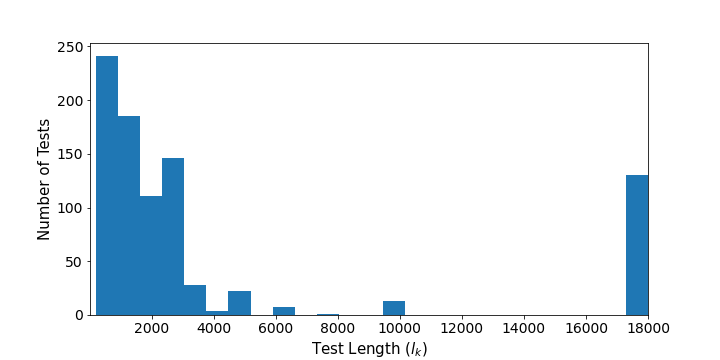
\includegraphics[width=\columnwidth]{ASE_files/test_lengths.png}
    % \Description[Number of tests histogram]{A histogram chart maxing on numbers less than 2,000 and over 17,500}
    \caption{Distribution of flight log lengths for the $N=888$ (out of the original 948 available logs) logs that were kept in the dataset ($200 \leq l_k \leq 20,000$)}
    \label{fig:test_lengths}
\end{figure}

% As mentioned before each input data item is a multivariate time series with $n=10$ variables (listed in table~\ref{tab:in_outs}). 
% During the data preprocessing, after the time series data is converted into tensors, all of the shorter $T_i$s were post-padded to the length of the longest one: $L=18000$ time steps.
The dataset was randomly split into three chunks of 90\%, 5\%, and 5\% for training, validation, and testing, where each sample corresponds to one test execution. Note that separate test and validation sets are needed to facilitate proper hyper-parameters tuning, without leaking information. 
% \subsection{System Under Study} \label{mp_data_collection}
% Our case study is a state-based system, which is real-time controller for UAVs, developed by
% our partner
% \begin{anonsuppress}
% Winnipeg based Micropilot Inc. Micropilot is the world-leader in professional UAV AutoPilot which develops both hardware and software for 1000+ clients (including NASA, Raytheon, and Northrop Grumman) in 85+ countries during the past 20+ years.
% \end{anonsuppress}
% .

%What the AutoPilot does can be summarized as `trying to hold some invariants based on the goal/state of the system'.
% % Maybe these two paragraphs can be moved somewhere more appropriate
% \label{changes_in_inputs}
% To work it backwards we capture the input/outputs (the UAV's relevant signals) over time and examine their correlations, i.e. how changes in one of them results in changes in another. When the state of the system changes these relations may change. So if we can capture what the relations are and when they change we can determine the state in which the system is in. 
% Of course pinpointing the exact moment when the changes happen is difficult; It is also impacted by the sampling time resolution so the inferred states and the change points are approximations.

\subsection{Experiment Execution Environment} \label{sec:machines_config}
Training and evaluation of the deep learning model was done on a single node running Ubuntu 18.04 LTS (Linux 5.3.0) equipped with Intel Core i7-9700 CPU, 32 gigabytes of main memory, and 8 gigabytes of GPU memory on a NVIDIA GeForce RTX 2080 graphics card.
The code was implemented using keras on TensorFlow 2.0.

The baseline models could not fit on that machine, so two nodes on Compute Canada's Beluga cluster, one with 6 CPUs and 75GiB of memory and one with 16 CPUs and 64GiB of memory, were used to train and evaluate them.

\subsection{Results} \label{sec:results}
In this section, we present the results of the experiments and answer the two research questions. 
\subsubsection{RQ1 Results: CPD Performance}
\begin{table*}
\caption{Change point detection precision, recall, and F1-score calculated for the baseline methods using three values of tolerance ($\tau$) for multiple configurations.}
\label{tab:rq1-results}
% TODO: change it to one of those large sideways tables \begin{landscape} \usepackage{lscape}
\resizebox{\textwidth}{!}{%
\begin{tabular}{llcccccccccc}
\toprule
  \textbf{Cost Function} &
  \textbf{Search Method} &
  \textbf{Penalty} &
  \textbf{Prec.} &
  \textbf{Recall} &
  \textbf{F1} &
  \textbf{Prec.} &
  \textbf{Recall} &
  \textbf{F1} &
  \textbf{Prec.} &
  \textbf{Recall} &
  \textbf{F1} \\
                                                  &              &   & \multicolumn{3}{c}{$\tau=1$s} & \multicolumn{3}{c}{$\tau=3$s} & \multicolumn{3}{c}{$\tau=5$s} \\  \toprule
\multirow{2}{*}{\textbf{Autoregressive Model}}     & Bottom Up    & 1000 & 10.43\%    & 75.44\%    & 18.33\%   & 21.21\%    & 80.32\%    & 33.55\%   & 28.94\%    & 81.22\%    & 42.68\%   \\
                                                   & Window Based & 100  & 2.94\%     & 3.98\%     & 3.38\%    & 8.53\%     & 11.41\%    & 9.76\%    & 12.89\%    & 17.54\%    & 14.86\%   \\ \midrule
\multirow{2}{*}{\textbf{Least Absolute Deviation}} & Bottom Up    & 500  & 7.32\%     & 52.54\%    & 12.85\%   & 17.52\%    & 87.73\%    & 29.20\%   & 25.02\%    & 88.95\%    & 39.05\%   \\
                                                   & Window Based & 500  & 5.24\%     & 8.31\%     & 6.42\%    & 15.20\%    & 24.03\%    & 18.62\%   & 21.79\%    & 38.25\%    & 27.76\%   \\ \midrule
\multirow{2}{*}{\textbf{Least Squared Deviation}}  & Bottom Up    & 1000 & 7.44\%     & 85.09\%    & 13.68\%   & 16.40\%    & 89.81\%    & 27.74\%   & 24.16\%    & 90.47\%    & 38.14\%   \\
                                                   & Window Based & 500  & 3.59\%     & 6.79\%     & 4.70\%    & 10.27\%    & 16.51\%    & 12.66\%   & 16.18\%    & 26.84\%    & 20.19\%   \\ \midrule
\multirow{2}{*}{\textbf{Linear Model Change}}      & Bottom Up    & 100  & \textbf{37.59\%}    & 28.98\%    & \textbf{32.73\%}   & \textbf{45.20\%}    & 38.39\%    & \textbf{41.52\%}   & \textbf{48.07\%}    & 41.36\%    & \textbf{44.46\% }  \\
                                                   & Window Based & 500  & 6.70\%     & 4.14\%     & 5.12\%    & 20.50\%    & 13.05\%    & 15.95\%   & 38.78\%    & 26.77\%    & 31.67\%   \\ \midrule
\multirow{2}{*}{\textbf{Gaussian Process Change}}  & Bottom Up    & 100  & 3.77\%     & \textbf{92.23\%}    & 7.25\%    & 8.99\%     & \textbf{92.23\%}    & 16.39\%   & 13.53\%    & \textbf{92.23\%}    & 23.60\%   \\
                                                   & Window Based & 100  & 2.94\%     & 3.95\%     & 3.37\%    & 8.69\%     & 11.50\%    & 9.90\%    & 13.64\%    & 18.30\%    & 15.63\%   \\ \midrule
\multirow{2}{*}{\textbf{Rank-based Cost Function}} & Bottom Up    & 100  & 13.45\%    & 60.19\%    & 21.98\%   & 19.49\%    & 80.10\%    & 31.35\%   & 22.98\%    & 87.23\%    & 36.38\%   \\
                                                   & Window Based & 100  & 8.10\%     & 13.70\%    & 10.18\%   & 15.72\%    & 30.73\%    & 20.80\%   & 21.38\%    & 46.64\%    & 29.32\%   \\ \midrule
\multirow{2}{*}{\textbf{Kernelized Mean Change}}   & Bottom Up    & 100  & 4.13\%     & 3.24\%     & 3.63\%    & 12.22\%    & 8.14\%     & 9.77\%    & 15.38\%    & 10.58\%    & 12.54\%   \\
                                                   & Window Based & 100  & 2.82\%     & 3.00\%     & 2.91\%    & 10.14\%    & 8.40\%     & 9.19\%    & 13.64\%    & 12.61\%    & 13.10\%   \\ \bottomrule

                                                   
\end{tabular}%
}
\end{table*}

Table~\ref{tab:rq1-results} shows the results of running CPD algorithms for various configurations (as described in \ref{sec:CPD_baseline}). For each search method and cost function pair only one of the penalty values which resulted in the highest F1 scores for all $\tau$ values is reported. 

The first observation from the results is that as values of $\tau$ increases the scores get better. This was expected, since larger values relax the constraints on which detected change points are considered as a true positive. Another observation is that the bottom-up segmentation consistently outperforms the window-based segmentation method. We can also see that the linear cost function beats all the other ones, in terms of precision. The Gaussian cost function achieves much higher recall values costing it a huge loss in precision. It means this cost function results in detecting numerous change points spread across the time axis, so there is a good chance of having at least one change point predicted close to each true change point (hence the high recall), but also there are a lot of false positives, which leads to a low precision. 

\begin{table}
\caption{Change point detection precision, recall, and F1-score calculated, on the test data, for our proposed model, using three values of tolerance ($\tau$) compared with the respective $\tau$'s best F1 score among baseline methods}
\label{tab:rq1-2-results}
% begin{tabular}{cccc}
\begin{tabularx}{\columnwidth}{cXXXX}
\toprule
  $\mathbf{\tau}$ &
  \textbf{Prec.} &
  \textbf{Recall} &
  \textbf{F1 score} & 
  \textbf{Baseline F1}  \\ \midrule
1s & 56.77\% &	79.32\% &	66.18\% & 32.73\% \\
3s & 69.58\% &	88.88\% &	78.06\% & 41.52\% \\
5s & 79.82\% &	91.87\%	&   85.42\% & 44.46\% \\\bottomrule
\end{tabularx}
%\end{tabular}
\end{table}

Measuring the same metrics on how our model performs on the test data shows better scores, almost twice the F1 score of the best performing baseline (see Table~\ref{tab:rq1-2-results}). Please note that unlike machine learning algorithms (such as ours), CPD algorithms do not have a separate training and testing phases. This fact works in their favor (by using the entire dataset for prediction and not just the training set), but still our model outperforms them.

%Although measuring the time it takes to detect change points was not one of the comparison metrics it would not hurt to note that
In terms of execution cost, running all 42 different settings of CPD algorithms on the whole dataset took a bit over 12 hours in the cloud using 16 CPUs and 64GB of main memory. The deep learning model on the other hand takes about an hour to train (which only needs to be done once), on a smaller machine (see section~\ref{sec:machines_config}). It made predictions on the whole dataset in less than a minute.
%$(/)-1=
So to answer RQ1, our method has shown $(66.18/32.73)-1=102.20\%$ improvement in F1 score with $\tau=1s$, $(78.06/41.52)-1=88.00\%$ with $\tau=3s$, and $(85.42/44.46)-1=92.13\%$ with $\tau=5s$; almost doubling the score compared to the baselines. 

\begin{rqanswer}
Our model, which requires less memory compared to traditional CPD algorithms, improved their best performance by up to 102\%, measured by F1 score, in less execution time.
\end{rqanswer}

\subsubsection{RQ2 Results: Multi-class Classification Performance}
To answer RQ2, we first compare different configurations of the baseline methods using the F1 score (harmonic mean of precision and recall) on the test data. The results are presented in Table~\ref{tab:rq2-1-results}.

\begin{table}
\caption{Precision, recall, and F1 score of ridge classifiers (linear classifiers with L2 regularization) and decision tree classifiers (DT) with different sliding window widths ($w$). For each algorithm on each $w$ several hyper-parameters were applied producing 152 different models. In this table, we only show the results of the best performing model in each group.}
\label{tab:rq2-1-results}
\resizebox{\linewidth}{!}{%
\begin{tabular}{clcclll}
\toprule
\textbf{w} &
  \multicolumn{1}{c}{\textbf{Classifier}} &
  \multicolumn{1}{c}{\textbf{\begin{tabular}[c]{@{}c@{}}Max\\ Depth\end{tabular}}} &
  \multicolumn{1}{c}{\textbf{\begin{tabular}[c]{@{}c@{}}Max\\ Features\end{tabular}}} &
  \multicolumn{1}{c}{\textbf{Prec.}} &
  \multicolumn{1}{c}{\textbf{Recall}} &
  \multicolumn{1}{c}{\textbf{F1}} \\ \midrule
3  & Ridge & -   & -          & 71.39\% & 20.73\% & 32.13\% \\
3  & DT    & -   & -          & 69.21\% & 82.36\% & 75.21\% \\ \midrule
5  & Ridge & -   & -          & 69.15\% & 21.89\% & 33.26\% \\
5  & DT    & 100 & -          & 68.37\% & \textbf{83.16\%} & 75.04\% \\ \midrule
10 & Ridge & -   & -          & 71.97\% & 24.02\% & 36.02\% \\
10 & DT    & 260 & -          & 67.94\% & 79.14\% & 73.12\% \\ \midrule
15 & Ridge & -   & -          & 76.87 & 25.90\% & 38.75\% \\
15 & DT    & -   & $\sqrt{10w}$ & 69.06\% & 80.76\% & 74.45\% \\ \midrule
20 & Ridge & -   & -          & \textbf{80.38\%} & 26.50\% & 39.86\% \\
20 & DT    & 175 & $\sqrt{10w}$ & 73.21\% & 82.16\% & \textbf{77.42\%} \\  \midrule
   & \multicolumn{3}{l}{Our Proposed Method} & \textbf{86.29\%} & \textbf{95.04\%} & \textbf{90.45\%} \\
\bottomrule
\end{tabular}%
}
\end{table}

Comparing the baseline methods with our proposed method (the last row) in Table~\ref{tab:rq2-1-results} shows that our model outperforms all baselines. Comparing it with the model with the best F1-score shows a $(86.29/73.21)-1=17.87\%$ improvement in precision as well as a $(95.04/82.16)-1=15.68\%$ improvement in recall that means $(90.45/77.42)-1=16.83\%$ overall improvement in F1-score. 

To have a feeling of how good our predictions are in practice, Figure~\ref{fig:test_0} shows the output of our model side by side with the ground truth. The horizontal axis shows sample ID (time) and the states are color coded. As it is seen, our algorithm performs better when the state changes are farther apart. Also there are some state changes that happen quite briefly which are not detected. That is not to a great surprise since it takes some time for state changes to be reflected in the outputs and those might not have got any chance.


The classical models only see one window of the data at a time, convolutional layers on the other hand are more generalized and flexible since each filter in each layer is comparable to a sliding window. As we saw in Table~\ref{tab:rq2-1-results}, a larger window size means a higher performance. However, it gets significantly more difficult to train a model with large window sizes. In addition, convolutions can automatically learn preprocessing steps that could be beneficial such as a moving average. Each convolutional filter can learn a linear combination of its inputs. So when the convolutional layers are stacked on each other, with non-linear activation functions in between, the hypothesis space they can learn becomes quite large, probably much larger than most of the classical ML algorithms here. Also, they are still quite efficient (more efficient than baselines) due to parameter sharing and their high parallelizability.

The fact that the performance improves as the window size increases indicates the positive effect of being able to see longer-term relations in detecting the system's state. Recurrent cells (such as GRU) can capture long-term dependencies (that do not necessarily fall into one window) and learn sequences. This is one of the major differences between an RNN model and others, such as decision trees, which do not have such a notion of a ``long-term memory'' as LSTM/GRU neural networks do. All a decision tree could see is the values in a sliding window.

In terms of the training complexity (time and memory), our method is superior as well. That can largely be attributed to the use of deep learning. In baseline models, as the window size $w$ grows the training and evaluation complexity grows, up to a point that they ran out of memory -- consuming all the 47GB of main memory and swap area. This forced us to train them in the cloud. Meanwhile, as mentioned earlier, the deep learning model could be trained on a 8GB GPU in roughly an hour. (see section \ref{sec:machines_config} for the machines' specs). Also, the decision tree training was not parallelized using only one core of the CPU, while virtually all deep learning models can be heavily parallelized on a GPU/TPU. %All the reported scores for both the baseline models and our model are computed on previously unseen test data. 

\begin{rqanswer}
Our model, which requires less than half as many CPUs and 70\% as much memory compared to the best performing classical ML model, improved their best performance by up to 17\%, measured by F1 score, in less execution time.
\end{rqanswer}


\begin{figure*}
    \centering
    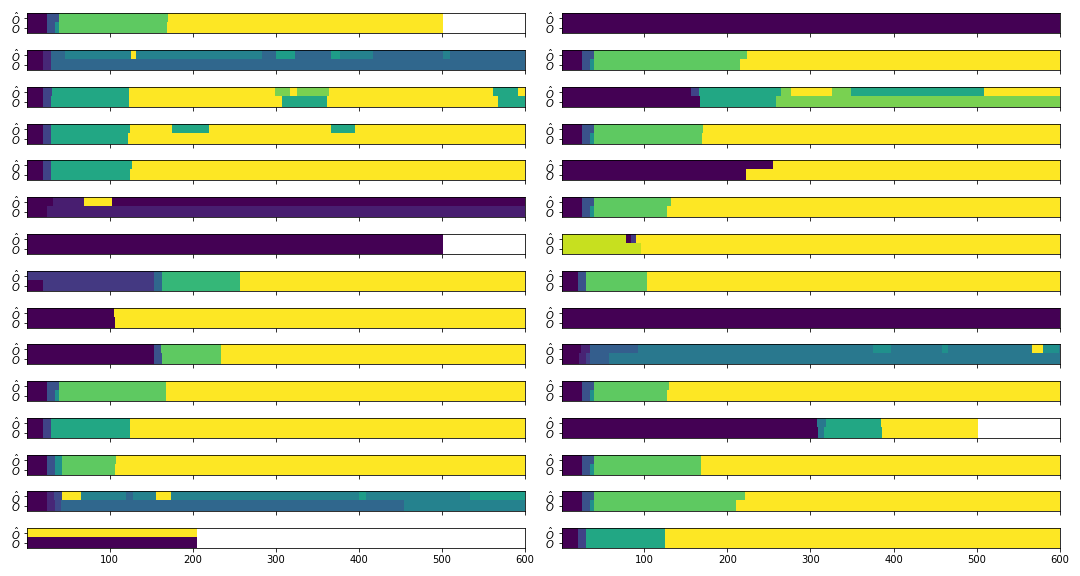
\includegraphics[width=\linewidth]{ASE_files/test_0.png}
    % \Description[States in time diagram]{A figure that color-codes the true and predicted states}
    \caption{Evaluation of the model on 30 random test data. Each graph shows the states in one run of the system. The colors show the states. The top-half of each plot depicts model's prediction of the system states ($\hat{O}$) and the bottom-half shows the true labels($O$). Since the output is one-hot encoded, the item with the most probability is used as the predicted label at each point in time. X-axis is the time axis. Only the first 600 samples (2 minute of simulation) are shown to improve legibility.}
    \label{fig:test_0}
\end{figure*}




\subsection{Limitations and Threats to Validity} \label{sec:threats_to_validity}
One of the limitations of our approach is that it might miss an input-output invariant correlation. It can happen when the input remains constant or it changes too little to reveal its relation with certain outputs. 
%In addition, as mentioned before, our approach relies on changes in signals. 
We assume that during the data collection, sampling happens in regular intervals; our approach probably will have a hard time achieving high performances, working on unevenly spaced time-series data.
%Maybe the CPD baselines could perform better if they were boosted by feature engineering, but the feature engineering task is can quickly become an arduous and inefficient. 
%It exists so it compensates for inability of traditional non-deep-learning methods in discovering meaningful features in the data. \cite{bengio2013deep}

In terms of construct validity, we are using standard metrics to evaluate the results. However, the use of tolerance margin should be taken with caution since it is a domain-dependant variable and can change the final results. To alleviate this threats, we have used multiple margins and reported all results. In terms of internal validity threats, we reduced the threat by not implementing the CPD baselines by ourselves and rather reusing existing libraries. In terms of conclusion validity threats, we have used many (888) real test cases from Micropilot's test repository and provided a proper train-validation-test split for training, tuning, and evaluation. Finally, in terms of external validity threats, our study suffers from being limited to only one case study. However, the study is a large-scale real-world study with many test cases. We plan to extend this work with more case studies from other domains, to increase its generalizability. 


 